The developed system is not completely autonomous, the first \acs{uav} has to fly to the \acs{qrcode} manually for the second \acs{uav} to fly to this without any other input than the location of the goal and the mapped environment.

There is currently no \acs{ros} algorithm for exploration in a \acs{3d} environment. Because of time constraints and lack of expertise, writing such an algorithm based on a \acs{2d} implementation is not realistic. The performance of Python is not adequate to run such an algorithm in real\hyp{}time, a language such as C++ should be used for this.

The path planning or exploration algorithm should be executed directly on the Octree output of \acs{rtabmap}. However, in this project, the Octree is converted to a \acs{3d} matrix to find the neighboring coordinates, which is an unnecessary conversion.

Because of developing in a simulated environment, the \acs{slam} algorithm detected loop closures where they should not be detected. The simulated environment is created with textures that repeat and are exactly the same each time, in a real environment two exactly the same textures do not exist. To overcome this issue, a different floor design was created where one texture with a lot of different colors was stretched over the whole surface to prevent the same detection at different locations. A better solution would be to create a more detailed simulated environment with custom textures or add random noise to each texture.

One of the biggest unsolved difficulties was to get the \acs{uav} to fly in a straight line over long distances. Two strategies of controlling the \acs{uav} were tested but both had the same result. One strategy was to send coordinates to the PX4 autopilot where it would fly to in a straight line, the other was sending velocity commands on every axis based on the desired location. In both cases, the \acs{uav} flew with a recurring deviation in its traveled path, visualized in figure~\ref{fig:deviation_path}. The blue line is the actual traveled path, the red line is the desired path.

\begin{figure}[!h]
  \centering
  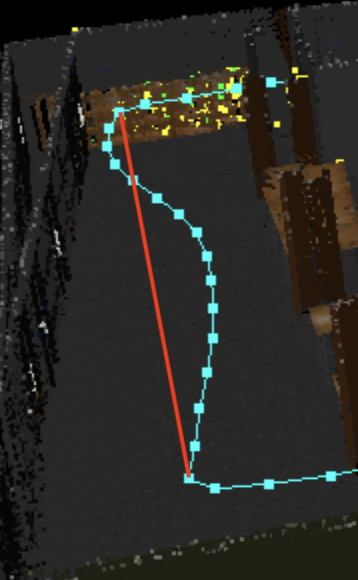
\includegraphics[height=0.27\linewidth]{images/deviation_path.png}
  \caption{Deviation on traveled path}
  \label{fig:deviation_path}
\end{figure}